\section{Summary and conclusions}\label{sec:summary}


We report on a first set of mass distributions and follow up diagnostics for 
the {\SW} lens candidates created with a novel approach that aims to be scalable 
by orders of magnitudes to prepare for the many thousands of lenses the next 
generation of wide field surveys will yield.

The way of discovering lenses is changing with the introduction of
machine learning and citizen science, combined with the coverage of
huge areas by modern surveys.  The way mass models are constructed also needs to
change, in order to be prepared for the increasing influx of lenses to
be modelled.  This work is a hybrid of the classical style, where a
small team of experts invest many hours into the creation of a single
model, with the approach of citizen science, where a crowd of amateur
volunteers make independent contributions.  We are a collaboration of
professionals and experienced citizen-science volunteers, aiming to
create early-stage lens models as soon as a lens candidate is found.

\begin{figure}
  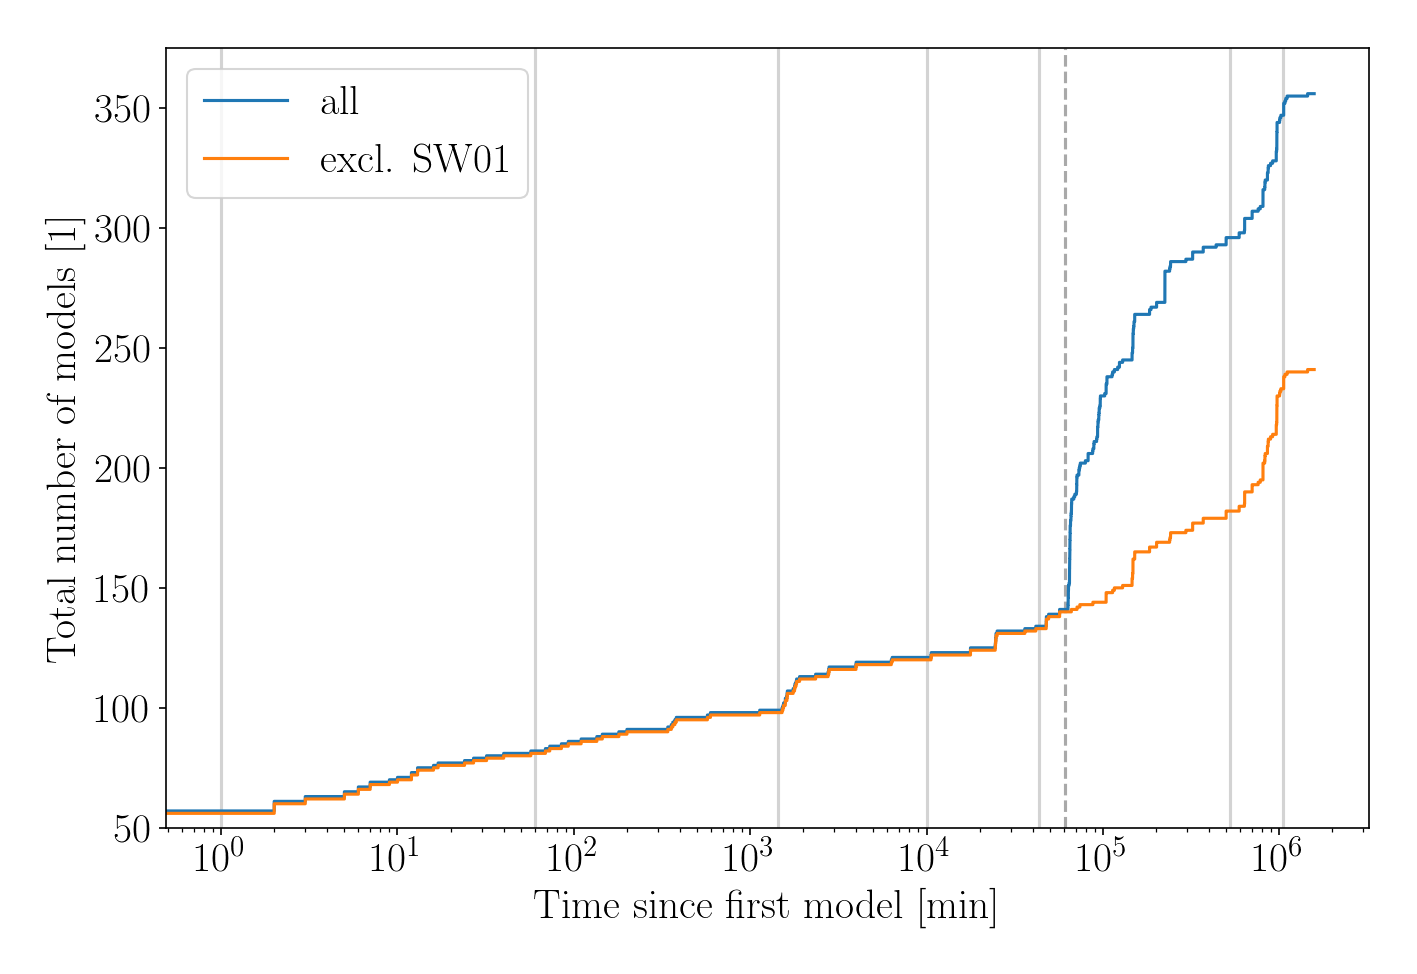
\includegraphics[width=\linewidth]{img/timelapse}
  \caption{Activity of volunteers; amount of models, summed over all candidates, after the first model was generated. 8 users contributed more than five models. vertical lines show 1 minute, one hour, one day, one week, one month, one year, two years. Dashed vertical line shows the start of the SW01 modelling challenge.}
  \label{fig:time}
\end{figure}



To assists volunteer modellers assessing their models, we introduce a
set of diagnostics allowing the qualification of the lenses and the
generated models and present them alongside the generated models. At a
later stage, we encourage modellers to apply those diagnostics
themselves to get a preliminary feedback on the plausibility of their
models and possibly suggest additional diagnostics.

The diagnostics (i) -- (iv) turned out to be useful for evaluating how difficult a system is to model, but they weren't necessary conditions for a promising model.
They can help select systems to present to novice volunteers to introduce them to the modelling process.
Diagnostics (v) and (vi) on the other hand can be considered as necessary criteria for a good model.
Volunteers employed those to evaluate their models and they turned out to be easy enough to grasp for new volunteers.
The halo-matching index $\haloindex$, diagnostic (vii), is an interesting criterion that might be useful for volunteers, but needs further investigation to be established.


Table~\ref{tab:models} is a summary of our results.  It characterises
each modelled system with seven diagnostics, indicating (a)~the image
morphology and how clear or indistinct it is, (b)~whether the mass map
and synthetic lensed image appear to be plausible, and (c)~how the
model mass compares with the estimated stellar and full-halo masses.
Missing entries are due to photometry data not being available, whereas
missing rows are due to models not having been created for this particular
candidate.

The trend in Figure~\ref{fig:stelmass}, that higher-mass galaxies get 
progressively more dark-matter dominated, is expected, e.g. see 
\cite{2005ApJ...623L...5F}, as is the span of about one order of magnitude for 
the stellar mass and the two order of magnitudes for the lensing mass. With 
future data, it would be interesting to compare enclosed stellar and lensing 
mass as a function of radius, going from star-dominated inner regions to dark 
halos. \cite{2011ApJ...740...97L} illustrate this behaviour in their Figure~5, 
but the present sample could go an order of magnitude higher in mass.

The quick creation of many models for the {\SW} candidates successfully showed 
that a subset of citizen scientists are interested in being involved in more 
challenging tasks that take some time to learn. A next steps involves 
recruiting more lensing enthusiasts, as soon as the next round of {\SW} is 
started. In the meantime, the improvements shown in the Appendix have to been 
integrated into regular {\SpL} usage. Additionally, photometric fitting could 
be integrated into {\SpL}. This would allow experienced citizen scientists to 
generate photometric redshifts and stellar masses, and thus generate 
preliminary dark-matter maps as soon as a lens-candidate is identified.

